\begin{frame}
    \titlepage
\end{frame}

\begin{frame}{logistical note}
    \begin{itemize}
    \item post-exam stack smashing assignment
    \item due two weeks after spring break (was one on schedule, but\ldots)
    \item likely harder than tricky --- will count for more
    \end{itemize}
\end{frame}

\begin{frame}{exam format}
    \begin{itemize}
    \item around 20 question parts
    \item mostly multiple choice or multiple-multiple choice
    \item something similar to RE
    \item something similar to TRICKY
    \item something about antiantivirus strategies, VMs, etc.
    \end{itemize}
\end{frame}

\begin{frame}{given information}
    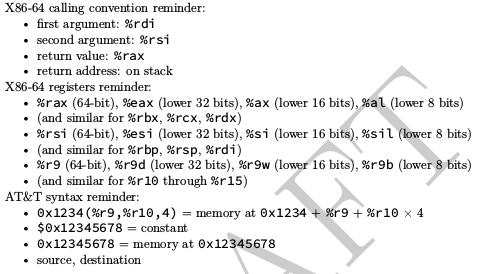
\includegraphics[width=0.85\textwidth]{exam-front-cheat}
\end{frame}


\section{virtual machines}

\begin{frame}{virtual machines}
    \begin{itemize}
    \item illusion of dedicated machine
    \item possibly different interface:
        \begin{itemize}
        \item system VM --- interface looks like some physical machine
        \item system VM --- OS runs inside VM
        \item process VM --- what OS implements
        \item process VM --- files instead of hard drives, threads instead of CPUs, etc.
        \item language VM --- interface designed for particular programming language
        \item language VM --- e.g. Java VM --- knows about objects, methods, etc.
        \end{itemize}
    \end{itemize}
\end{frame}

\begin{frame}{virtual machine implementation techniques}
    \begin{itemize}
    \item emulation:    
        \begin{itemize}
        \item read instruction + giant if/else if/\ldots
        \end{itemize}
    \item binary translation
        \begin{itemize}
        \item compile machine code to new machine code
        \end{itemize}
    \item ``native''
        \begin{itemize}
        \item run natively on hardware in user mode
        \item hardware triggers ``exceptions'' on special interrupts
        \item exceptions give VM implementation control
        \end{itemize}
    \end{itemize}
\end{frame}

\begin{frame}{VM implementation strategies}
    \begin{tikzpicture}
    \begin{scope}[yscale=0.75,xscale=1.5]
    \node[anchor=center] at (3, .5) {\bfseries traditional VM};
    \draw[thick] (0, 0) -- (6, 0) -- (6, -1) -- (3, -1) -- (3, -2)  -- (1, -2) -- (1, -3) -- (0, -3) -- cycle;
    \node[anchor=center] at (3, -.5) {virtual machine/guest OS};
    \draw[thick] (6, -3) -- (6, -1) --  (3, -1) -- (3, -2) --  (5, -2) -- (5, -3) -- cycle;
    \node[anchor=center] at (4.5, -1.5) {VM monitor};
    \draw[thick] (1, -2) -- (1, -3) -- (5, -3) -- (5, -2) -- cycle;
    \node[anchor=center] at (3, -2.5) {host OS};
    \draw[thick] (0, -3) -- (0, -4) -- (6, -4) -- (6, -3) -- cycle;
    \node[anchor=center] at (3, -3.5) {native CPU};
    \begin{visibleenv}<2->
        \draw[very thick, orange] (3, -1) -- (6, -1) node[right,orange,align=center] {privileged ops \\ become callbacks \\ (help from HW+OS)};
        %\draw[very thick, red] (5, -2) -- (1, -2) node[left,red,align=center] {system\\ calls};
        \draw[very thick, blue] (0, -3) -- (6, -3) node[right,blue] {native instruction set};
    \end{visibleenv}
        \coordinate (sameNativeLine) at (3, -3);
        \begin{pgfonlayer}{fg}
        \begin{visibleenv}<3>
        \node[mycallout2=sameNativeLine,anchor=north,align=left] at (3, -4) {
            virtual ISA same as real ISA \\
            (except for privileged operations)
        };
        \end{visibleenv}
        \end{pgfonlayer}
    \end{scope}
    \begin{scope}[yshift=-3.7cm,xscale=1.5,yscale=0.75]
    \node[anchor=center] at (3, .5) {\bfseries emulator};
    \draw[thick] (0, 0) -- (6, 0) -- (6, -1) -- (0, -1) -- cycle;
    \node[anchor=center] at (3, -.5) {virtual machine/guest OS};
    \draw[thick] (6, -1) -- (0, -1) -- (0, -2)  -- (5, -2) -- (5, -3) -- (6, -3) -- cycle;
    \node[anchor=center] at (3, -1.5) {emulator};
    \draw[thick] (0, -2) -- (0, -3) -- (5, -3) -- (5, -2) -- cycle;
    \node[anchor=center] at (3, -2.5) {host OS};
    \draw[thick] (0, -3) -- (0, -4) -- (6, -4) -- (6, -3) -- cycle;
    \node[anchor=center] at (3, -3.5) {native CPU};
    \begin{visibleenv}<2->
        \draw[very thick, red] (0, -1) -- (6, -1) node[right,red,align=center] {interpret/translate};
        \draw[very thick, blue] (0, -3) -- (6, -3) node[right,blue] {native instruction set};
    \end{visibleenv}
    \begin{visibleenv}<4>
        \coordinate (diffNativeLine) at (3, -1);
        \node[mycallout2=diffNativeLine,anchor=south,align=left] at (4, 0) {
            virtual ISA could be different from real ISA \\
            (even excluding privileged operations)
        };
    \end{visibleenv}
    \end{scope}
    \end{tikzpicture}
\end{frame}

\begin{frame}{system call flow}
\begin{tikzpicture}
\tikzset{
    userProg/.style={fill=green!20!white},
    innerOS/.style={fill=blue!20!white},
    outerOS/.style={fill=yellow!20!white},
}
\matrix[tight matrix,nodes={align=center,text width=9cm,minimum height=1.7cm,execute at begin node=\strut},
    label={[inner sep=1mm]north:conceptual layering}] (layering) {
    |[userProg]| {program \\ ~} \\
    |[innerOS]| {`guest' OS \\ ~} \\
    |[outerOS]| {virtual machine monitor \\ ~} \\
    hardware \\
};
\begin{visibleenv}<3>
    \node[draw,line width=1mm,blue,fit=(layering-1-1) (layering-2-1),inner sep=-.25mm,
        label={[align=left,blue!80!black]right:user\\mode}] {}; 
    \node[draw,line width=1mm,red,fit=(layering-3-1),inner sep=-.25mm,
        label={[align=left,red!80!black]right:kernel\\mode}] {}; 
\end{visibleenv}
\begin{visibleenv}<2,6>
    \node[draw,line width=1mm,cyan,fit=(layering-1-1),inner sep=-.25mm,
        label={[align=left,cyan!80!black]right:pretend\\user\\mode}] {}; 
    \node[draw,line width=1mm,magenta,fit=(layering-2-1),inner sep=-.25mm,
        label={[align=left,magenta!80!black]right:pretend\\kernel\\mode}] {}; 
\end{visibleenv}
\begin{visibleenv}<4->
\begin{scope}
    \tikzset{
        >=Latex,
        l/.style={very thick,red!90!black},
        every node/.style={
            inner sep=1mm
        }
    }   
    \draw[l,->] ([xshift=-8cm,yshift=.1cm]layering-1-1.south east) -- ([xshift=-7.5cm,yshift=-.4cm]layering-4-1.north east)
        node[above,at start,align=center,xshift=3mm] {system call\\(exception)};
    \draw[l,->] ([xshift=-7cm,yshift=-.4cm]layering-4-1.north east) -- ([xshift=-6.6cm,yshift=.1cm]layering-3-1.south east)
        node[above,xshift=.5cm] { \textbf<5>{run handler} };
    \draw[l,->] ([xshift=-5cm,yshift=.1cm]layering-3-1.south east) -- ([xshift=-4.5cm,yshift=-.2cm]layering-4-1.north east)
        -- ([xshift=-4cm,yshift=.1cm]layering-3-1.south east)
        node[below,midway,align=left] { \textbf<6>{update memory map} };
    \draw[l,->] ([xshift=-2cm,yshift=.1cm]layering-3-1.south east) -- ([xshift=-1.5cm,yshift=-.2cm]layering-4-1.north east)
        node[at start,above left,xshift=.5cm,align=left] {to user mode}
        -- ([xshift=-.8cm,yshift=.1cm]layering-2-1.south east)
        node[at end,above,xshift=-.5cm] { \textbf<5>{run handler} };
\end{scope}
\end{visibleenv}
\end{tikzpicture}
\end{frame}

\begin{frame}{VMs and malware}
    \begin{itemize}
    \item isolate malware from important stuff
    \item sample malware behavior
        \begin{itemize}
        \item inspect memory for patterns --- counter for metamorphic
        \item look for suspicious behavior generally
        \end{itemize}
    \end{itemize}
\end{frame}

\begin{frame}{counter-VM techniques}
    \begin{itemize}
    \item detect VM-only devices
    \item outrun patience of antivirus VM
    \item unsupported instructions/system calls
    \item \ldots
    \end{itemize}
\end{frame}

\begin{frame}{debugger support}
    \begin{itemize}
    \item hardware support:
    \vspace{.5cm}
    \item breakpoint instruction --- debugger edits machine code to add
    \item single-step flag --- execute one instruction, jump to OS (debugger)
    \end{itemize}
\end{frame}

\begin{frame}{counter-debugger techniques}
\begin{itemize}
\item debuggers --- also for analysis of malware
\vspace{.5cm}
\item detect changes to machine code in memory
\item directly look for debugger
    \item broken executables
    \item \ldots
    \end{itemize}
\end{frame}
\section{assembly}

\begin{frame}[fragile,label=att1]{AT\&T syntax}
\begin{lstlisting}
movq $42, 100(%rbx,%rcx,4)
\end{lstlisting}
    \begin{itemize}
    \item destination \myemph{last}
    \item constants start with {\tt \$}; no {\tt \$} is an address
    \item registers start with {\tt \%}
    \item operand length ({\tt q} = 8; {\tt l} = 4; {\tt w} = 2; {\tt b} = 1)
    \item {\tt D(R1,R2,S)} = memory at {\tt D + R1 + R2 $\times$ S}
    \end{itemize}
\end{frame}

\begin{frame}{weird x86 features}
    \begin{itemize}
    \item segmentation: old way of dividing memory: {\tt \%fs:0x28} 
        \begin{itemize}
        \item get segment \# from FS register
        \item lookup that entry in a table
        \item add {\tt 0x28} to base adddress in table
        \item access memory as usual
        \end{itemize}
    \item rep prefix
        \begin{itemize}
        \item repeat instruction until rcx is 0
        \item \ldots decrementing rcx each time
        \end{itemize}
    \item string instructions
        \begin{itemize}
        \item memory-to-memory; designed to be used with rep/etc. prefixes
        \end{itemize}
    \end{itemize}
\end{frame}

\section{executable formats}

\begin{frame}[fragile,label=execParts]{executable/object file parts}
    \begin{tikzpicture}
    \tikzset{
        every node/.style={align=center},
    }
    \draw[very thick,fill=violet!20] (0, 0) rectangle (15, -1) 
    node[midway] {
        type of file, entry point address, \ldots
    };
    \draw[very thick] (0, -1) rectangle (15, -3) 
    node[midway] {
        \begin{tabular}{lllll}
        seg\# & file offset & memory loc. & size & permissions \\
        1 & {\tt 0x0123} & {\tt 0x3000} & {\tt 0x1200} & read/exec \\
        2 & {\tt 0x1423} & {\tt 0x5000} & {\tt 0x5000} & read/write \\
        \end{tabular}
    };
    \draw[very thick,fill=blue!20] (0, -3) rectangle (15, -4.5)
    node[midway,font=\large] {
        machine code + data for segments
    };
    \draw[very thick,fill=green!20] (0, -4.5) rectangle (15, -7)
    node[midway] {
        \textbf{symbol table}: {\tt foobar} at {\tt 0x2344}; {\tt barbaz} at {\tt 0x4432}; \ldots \\
        \textbf{relocations}: {\tt printf} at {\tt 0x3333} (type: absolute); \ldots \\
        section table, debug information, etc.
    };
    \end{tikzpicture}
\end{frame}

\begin{frame}{relocations?}
    \begin{itemize}
    \item unknown addresses --- ``holes'' in machine code/etc.
    \item linker lays out machine code
    \item computes all symbol table addresses
    \item uses symbol table addresses to fill in machine code
    \end{itemize}
\end{frame}

\begin{frame}[fragile,label=dynamicStubs]{dynamic linking}
    \begin{itemize}
    \item executables not completely linked --- library loaded at runtime
    \item could use same mechanism, but ineffecient
    \item instead: stubs:
    \end{itemize}
\begin{Verbatim}[commandchars=Q\{\},fontsize=\fontsize{8}{9}\selectfont]
0000000000400400 <puts@plt>:
  400400:	ff 25 12 0c 20 00    	jmpq   *0x200c12(%rip) 
                    /* 0x200c12+RIP = _GLOBAL_OFFSET_TABLE_+0x18 */
Qtextit{... later in main: ...}
  40052d:	e8 ce fe ff ff       	callq  400400 <puts@plt>
                        /* instead of call puts */
\end{Verbatim}
\end{frame}

\section{malware definitions}

\begin{frame}{malware}
    \begin{itemize}
    \item \myemph{evil software}
    \vspace{.5cm}
    \item various kinds:
        \begin{itemize}
        \item viruses
        \item worms
        \item trojan (horse)s
        \item potentially unwanted programs/adware
        \item rootkits
        \item logic bombs
        \end{itemize}
    \end{itemize}
\end{frame}

\begin{frame}{worms}
    \begin{itemize}
    \item malicious program that copies itself
    \item arranges to be run automatically (e.g. startup program)
    \item may spread to other media (USB keys, etc.)
    \item may spread over the network using vulnerabilities
    \end{itemize}
\end{frame}

\subsection{viruses and virus techniques}

\begin{frame}{viruses}
    \begin{itemize}
    \item malware that embeds itself in innocent programs/files
    \item spreads (primarily) by:
        \begin{itemize}
        \item hoping user shares infected files
        \end{itemize}
    \end{itemize}
\end{frame}

\begin{frame}{code placement options}
\begin{tikzpicture}[scale=0.5,transform shape]
    \tikzset{every node/.style={font=\Large}}
    \begin{scope}
    \draw[thick] (0, 0) rectangle (4, -6) node[midway,align=center] {original\\executable};
    \draw[line width=2mm,-Latex,black!60] (4.1, -3) -- (6.9, -.5);
    \begin{scope}[xshift=7cm]
    \draw[thick,fill=red!20] (0, 0) rectangle (4, -1) node[midway,align=center] {virus code};
    \draw[thick,fill=yellow!20] (0, -1) rectangle (4, -1.5) node[midway,align=center,font=\scriptsize] {
        run original from tempfile
    };
    \draw[thick] (0, -1.5) rectangle (4, -7.2) node[midway,align=center] {original\\executable};
    \end{scope}
    \end{scope}

    \begin{scope}[xshift=16cm]
    \draw[thick] (0, 0) rectangle (4, -5) node[midway,align=center] {original\\executable};
    \draw[line width=2mm,-Latex,black!60] (4.1, -3) -- (6.9, -3);
    \begin{scope}[xshift=7cm]
    \draw[thick] (0, 0) rectangle (4, -5) node[midway,align=center] {original\\executable};
    \draw[fill=red!20,thick] (0, -5) rectangle (4, -6)
        node[midway,align=center] {virus code};
    \draw[fill=red!20,thick] (0.5, -1) rectangle (1, -1.5);
    \node[anchor=west,red!50!black] at (1.25, -1.25) {jmp to virus};
    \draw[thick,Latex-] (1, -1.25) -- (1.4, -1.25);
    \end{scope}
    \end{scope}

    \begin{scope}[yshift=-8cm]
    \draw[thick] (0, 0) rectangle (4, -6) node[midway,align=center] {original\\executable};
    \draw[line width=2mm,-Latex,black!60] (4.1, -3) -- (6.9, -3);
    \begin{scope}[xshift=7cm]
    \draw[fill=red!20,thick] (0, 0) rectangle (4, -1) node[midway] {virus code};
    \draw[fill=red!20,thick] (0, -1) rectangle (4, -2) node[midway] {decompressor};
    \draw[pattern=north west lines,pattern color=black!70,thick] (0, -2) rectangle (4, -5)
        node[midway,fill=white,align=center] {compressed \\ executable};
    \draw[fill=black!60,thick] (0, -5) rectangle (4, -6)
        node[midway,white] {unused space};
    \end{scope}
    \end{scope}
   
    \begin{scope}[yshift=-8cm,xshift=16cm] 
    \draw[thick] (0, 0) rectangle (4, -6) node[midway,align=center,yshift=1.5cm] {original\\executable\\ (w/ cavities)};
        \draw[pattern=north west lines] (0, -3) rectangle (4, -3.5);
        \draw[pattern=north west lines] (0, -4) rectangle (4, -4.5);
        \draw[pattern=north west lines] (0, -5) rectangle (4, -5.5);
    \draw[line width=2mm,-Latex,black!60] (4.1, -3) -- (6.9, -3);
    \begin{scope}[xshift=7cm]
        \draw[fill=red!20,thick] (0, 0) rectangle (4, -0.5) node[midway] {startup code};
        \draw[fill=red!20,thick] (0, -0.5) rectangle (4, -1) node[midway] {code locs};
        \draw[thick] (0, -1) rectangle (4, -6);
        \draw[fill=red!20,thick] (0, -3) rectangle (4, -3.5)
            node[midway] {virus part 1};
        \draw[fill=red!20,thick] (0, -4) rectangle (4, -4.5)
            node[midway] {virus part 2};
        \draw[fill=red!20,thick] (0, -5) rectangle (4, -5.5)
            node[midway] {virus part 3};
    \end{scope}
    \end{scope}
\end{tikzpicture}
\end{frame}

\begin{frame}{entry point choices}
    \begin{itemize}
    \item entry address
        \begin{itemize}
        \item perhaps a bit obvious
        \end{itemize}
    \item overwrite machine code and restore
    \item edit call/jump/ret/etc.
        \begin{itemize}
        \item pattern-match for machine code
        \item in dynamic linking ``stubs''
        \item in symbol tables
        \item call/ret at end of virus
        \end{itemize}
    \end{itemize}
\end{frame}

\section{anti-virus and anti-anti-virus techniques}

\begin{frame}{pattern matching}
    \begin{itemize}
    \item regular expressions --- (almost) one-pass
    \item fixed strings with ``wildcards''
        \begin{itemize}
        \item addresses/etc. that change between instances of malware
        \item insert nops/variations on instructions
        \end{itemize}
    \end{itemize}
\end{frame}

\usetikzlibrary{arrows,automata}
\begin{frame}[fragile,label=flexHow]{flex: state machines}
\lstset{
        style=small,
        language={},
        moredelim={**[is][\btHL<2|handout:0>]{@hi2@}{@endhi@}},
        }
\begin{tikzpicture}
\node (flexStuff) {
\begin{lstlisting}
foo     {...}
.       {...}
\n      {...}
\end{lstlisting}
};
\begin{scope}[every node/.style={font=\tt,thick}]
\node[initial, state,below=1cm of flexStuff,font=\normalfont\it] (start) {};
\node[state,right=1cm of start] (f) {f};
\node[state,right=1cm of f] (fo) {fo};
\node[state,right=1cm of fo,accepting] (foo) {foo};
\node[state,below right=2cm of start,accepting] (dot) {.};
\node[state,below=1.5cm of start,accepting] (newline) {\textbackslash{}n};
\end{scope}
\path[-Latex,thick] (start) edge node[above] {\tt f} (f)
                    (f) edge node[above] {\tt o} (fo)
                    (fo) edge node[above] {\tt o} (foo)
                    (start) edge node[sloped,above] {other} (dot)
                    (start) edge node[left] {\textbackslash{}n} (newline);
\begin{visibleenv}<2>
    \path[-Latex,blue,dashed] (f) edge node[right] {(back 1)} (dot);
    \path[-Latex,blue,dashed] (fo) edge[out=-45,in=-30] node[midway, sloped, below] {(back 2)} (dot);
\end{visibleenv}
\end{tikzpicture}

\end{frame}

\begin{frame}{behavior-based detection/blocking}
    \begin{itemize}
    \item modifying executables? etc.
    \item must be malicious
    \end{itemize}
\end{frame}

\begin{frame}{armored viruses, etc.}
    \begin{itemize}
    \item evade analysis: 
        \begin{itemize}
        \item ``encrypt'' code (break disassembly)
        \item detect/break debuggers
        \item detect/break VMs
        \end{itemize}
    \item evade signatures:
        \begin{itemize}
        \item \myemph{oligomorphic/polymorphic}: varying ``decrypter''
        \item \myemph{metamorphic}: varying ``decrypter'' and varying ``encrypted'' code
        \end{itemize}
    \item evade active detection:
        \begin{itemize}
        \item \myemph{tunnelling} --- skip anti-virus hooks
        \item \myemph{stealth} --- `hook' system calls to say ``executable/etc. unchanged''
        \item \myemph{retroviruses} --- break/uninstall/etc. anti-virus software
        \end{itemize}
    \end{itemize}
\end{frame}

\begin{frame}<1>[fragile,label=caseEvol]{case study: Evol}
    \begin{itemize}
    \item via Lakhatia et al, ``Are metamorphic viruses really invincible?'', Virus Bulletin, Jan 2005.
    \item ``\myemph{mutation engine}''
        \begin{itemize}
        \item run as part of propagating the virus
        \end{itemize}
    \end{itemize}
    \begin{tikzpicture}
        \tikzset{
            every node/.style={font=\small,align=center},
            hiOn/.style={alt=<#1>{red,ultra thick}{}},
        }
        \path node[draw,hiOn=2] (disasm) {disassemble} -- ++(2.5cm,0) node (lens) {instr. \\ lengths} -- ++(2cm,0) node[draw,hiOn=3] (xform) {transform}
              -- ++(2cm,0) node[draw,hiOn=4] (reloc) {relocate};
        \node (origCode) at ([xshift=-2cm,yshift=1cm]disasm.north) {code};
        \node (finalCode) at ([xshift=2cm,yshift=-1cm]reloc.south) {code};
        \begin{scope}[thick,-Latex]
        \draw (origCode) |- (disasm);
        \draw (disasm) -- (lens);
        \draw (lens) -- (xform);
        \draw (xform) -- (reloc);
        \end{scope}
    \end{tikzpicture}
\end{frame}

\begin{frame}<1>[label=hookingList]{hooking mechanisms}
    \begin{itemize}
    \item hooking --- getting a `hook' to run on (OS) operations
        \begin{itemize}
        \item e.g. creating new files
        \end{itemize}
    \item ideal mechanism: \myemph<2>{OS support}
    \item less ideal mechanism: \myemph<3>{change library loading}
        \begin{itemize}
        \item e.g. replace `open', `fopen', etc. in libraries
        \end{itemize}
    \item less ideal mechanism: \myemph<4>{replace OS exception} (system call) handlers
        \begin{itemize}
        \item very OS version dependent
        \end{itemize} 
    \end{itemize}
\end{frame}


\section{vulnerabilities}

\begin{frame}{software vulnerabilities}
    \begin{itemize}
    \item unintended program behavior an adversary can use
    \vspace{.5cm}
    \item \myemph{memory safety bugs}
        \begin{itemize}
        \item especially buffer overflows
        \end{itemize}
    \item not checking inputs/permissions
    \item injection/etc. bugs
    \end{itemize}
\end{frame}

\section{exploits and stack smashing}

\begin{frame}{exploits}
    \begin{itemize}
    \item something that uses a vulnerability to do something
    \item example: stack smashing --- exploit for stack buffer overflows
    \end{itemize}
\end{frame}

\begin{frame}[fragile,label=returnToStack]{return-to-stack}
\begin{tikzpicture}
\tikzset{
    stackBox/.style={very thick},
    onStack/.style={thick},
    xscale=1.3,
}
\draw[stackBox] (0, 0) rectangle (10, -6);
\draw[thick,-Latex] (10.25,-5) -- (10.25, -1) node [midway, below, sloped] {increasing addresses};
\node[inner sep=0mm,at={(5, 0.1)},anchor=south] { highest address (stack started here)};
\node[inner sep=0mm,at={(5, -6.1)},anchor=north] { lowest address (stack grows here)};

\draw[onStack] (0, -.25) rectangle (10, -1.25) node[midway,align=center,font=\small] (stackAddr)
     {return address for {\tt vulnerable}: \\ \fontsize{10}{11}\selectfont\tt\bfseries\color{red}70 fd ff ff  ff ff 00 00 (0x7fff ffff fd70)};
\draw[onStack,fill=black!20] (0, -1.25) rectangle (10, -2.25) node[midway,align=center,font=\small] {unused space (20 bytes)};
\draw[onStack,fill=blue!20] (0, -2.25) rectangle (10, -5.25) node[midway,align=center,font=\small] {buffer (100 bytes)};

\draw[onStack] (0, -5.25) rectangle (10, -6) node[midway,align=center,font=\small] {return address for {\tt scanf}};

\begin{visibleenv}<2>
\draw[-Latex,red,ultra thick] ([yshift=2.5mm]stackAddr.south east) -- ++(.25cm,0cm) |- (0.25, -5);
\node[anchor=south west,red] at (0.25, -4.75) {
    machine code for the attacker to run
};
\end{visibleenv}

\end{tikzpicture}
\end{frame}
